% !TeX spellcheck = nb_NO
% Kommentaren ovenfor gir instruks til editoren din om at den skal bruke norsk stavekontroll. Dette fungerer bl.a. i TeXstudio.

\documentclass[a4paper,norsk]{article}
% Norsk orddeling
\usepackage[norsk]{babel}
% AMS-pakkene er nyttige
\usepackage{amsmath,amsfonts,amssymb,amsthm}
% For å definere lister, som f.eks. deloppgaver
\usepackage{enumitem}
% Inneholder mye nyttig, slik som \coloneqq
\usepackage{mathtools}
% Penere kalligrafiske fonter
\usepackage[utf8]{inputenc}
\usepackage[T1]{fontenc}
\usepackage[a4paper, margin=0.5in]{geometry}
\usepackage{mathabx}
\usepackage{amsthm}
\usepackage{listings}
\usepackage{xcolor}
\usepackage{ifthen}
\usepackage{hyperref}

\usepackage[most]{tcolorbox}
\tcbuselibrary{theorems, breakable}
\tcbset{before upper=\par, after upper=\par} % allows itemize and enumerate inside boxes

\newtcbtheorem[]{definitionbox}{Definisjon}{
  colback=blue!3,
  colframe=blue!70!black,
  fonttitle=\bfseries\color{white},
  coltitle=white,
  boxrule=0.6pt,
  arc=2mm,
  enhanced,
  breakable
}{def}

\newtcbtheorem[]{theorembox}{Teorem}{
  colback=green!3,
  colframe=green!50!black,
  fonttitle=\bfseries,
  coltitle=black,
  boxrule=0.6pt,
  before upper=\par\ignorespaces,
  after upper=\par\unskip,
  arc=2mm,
  enhanced,
  breakable
}{thm}

\newtcbtheorem[]{oppgavebox}{Oppgave}{
  colback=gray!5,
  colframe=black!60,
  fonttitle=\bfseries,
  coltitle=black,
  boxrule=0.6pt,
  arc=2mm,
  enhanced,
  breakable
}{oppg}

\newtcolorbox{sectionbox}[1][]{
  colback=white,
  colframe=black!70,
  boxrule=0.7pt,
  arc=3mm,
  top=2mm, bottom=2mm, left=2mm, right=2mm,
  title=#1,
  enhanced,
  breakable
}

\newtcbtheorem[]{corollarybox}{Korollar}{
  colback=purple!5,
  colframe=purple!60!black,
  fonttitle=\bfseries\color{white},
  coltitle=white,
  boxrule=0.6pt,
  arc=2mm,
  enhanced,
  breakable,
  before upper=\par\ignorespaces,
  after upper=\par\unskip
}{cor}

\newtcbtheorem[]{lemmabox}{Lemma}{
  colback=orange!5,
  colframe=orange!70!black,
  fonttitle=\bfseries,
  boxrule=0.6pt,
  arc=2mm,
  enhanced,
  breakable
}{lem}

\newtcbtheorem[]{propositionbox}{Proposisjon}{
  colback=cyan!5,
  colframe=cyan!60!black,
  fonttitle=\bfseries,
  coltitle=black,
  boxrule=0.6pt,
  arc=2mm,
  enhanced,
  breakable
}{prop}

\newtcbtheorem[]{proofbox}{Bevis}{
  colback=white,
  colframe=black,
  fonttitle=\bfseries\color{white},
  coltitle=white,
  colbacktitle=black,
  title style={opacity=0.9},
  boxrule=0.6pt,
  arc=2mm,
  enhanced,
  breakable
}{proofbox}

\newlist{suboppgave}{enumerate}{1}
\setlist[suboppgave,1]{
  label=\textbf{(\alph*)},
  ref=\theenumi\alph*,
  leftmargin=1.5em,
  itemsep=0.4em,
  topsep=0.3em,
  parsep=0pt,
  partopsep=0pt
}



\setcounter{secnumdepth}{2}  % Sections and subsections numbered

% Python style  
\lstdefinestyle{pythonstyle}{
    language=Python,
    basicstyle=\ttfamily\small,
    keywordstyle=\color{blue},
    commentstyle=\color{green},
    numbers=left,
    frame=single
}

% Bruk bedre symboler for ≥, ≤, epsilon og phi
\renewcommand{\geq}{\geqslant}
\renewcommand{\leq}{\leqslant}
\newcommand{\eps} {\varepsilon}
\renewcommand{\epsilon}{\varepsilon}
\renewcommand{\phi}{\varphi}

% Definer de vanligste mengdene og funksjonene
\newcommand{\R}{\mathbb{R}}
\newcommand{\K}{\mathbb{K}}
\newcommand{\C}{\mathbb{C}}
\newcommand{\N}{\mathbb{N}}
\newcommand{\Z}{\mathbb{Z}}
\newcommand{\Q}{\mathbb{Q}}
% \L er definert som noe annet fra før av, så vi må redefinere \L
\renewcommand{\L}{\mathcal{L}}
% Rommet av polynomer
\newcommand{\Pol}{{\mathcal{P}}}
\DeclareMathOperator{\id}{id}
\DeclareMathOperator{\Image}{im}
\DeclareMathOperator{\Kernel}{ker}
\DeclareMathOperator{\Span}{span}
\DeclareMathOperator{\Rank}{rank}
\DeclareMathOperator{\Diag}{diag}
\DeclareMathOperator{\Proj}{proj}
\newcommand{\basis}{{\mathcal{B}}}
\newcommand{\basiss}{{\mathcal{C}}}
\newcommand{\basisss}{{\mathcal{D}}}

\usepackage[most]{tcolorbox}
\newtcolorbox{algoritme}[1]{
  title=Algoritme~#1,
  colback=white,
  colframe=black,
  boxrule=0.5pt,
  arc=2mm,
  left=3mm,
  right=3mm,
  top=1mm,
  bottom=1mm
}

% Definer oppgavemiljøet
\newenvironment{oppgave}[1]%
	{\trivlist{}\item\relax\textbf{Løsning på #1.}\medspace}%
	{\endtrivlist}
% Deloppgavelister
\newlist{deloppgave}{enumerate}{1}
\setlist[deloppgave,1]{label=(\textbf{\alph*}),align=left}

\title{Oblig 5 \\ MAT1125, høst 2025}
\author{Oliver Ekeberg}
\begin{document}
\maketitle

\tableofcontents


\section*{5.6 Singulærverdidekomposisjon}
\addcontentsline{toc}{section}{5.6 Singulærverdidekomposisjon}

\begin{lemmabox}{5.6.1}{}
    La U og V være endeligdim indreproduktrom, og la $ T \in \mathcal{L}(U, V) $. Operatoren $ T^*T \in \mathcal{L}(U) $
    
    \begin{itemize}
        \item Er selvadjungert $ \left( T = T^* \right)  $ 
        \item Har relle, ikke negative egenverdier (\textbf{\textit{positiv semidefinitt}})
        \item $ kerT = ker T^*T $ og $ imT^* = imT^*T $  
    \end{itemize}
\end{lemmabox}

\begin{proofbox}{lemma 5.6.1}{}
Skal vise i) at $ T^* T $ er selvadjungert. Det skjer om
\[
    T^*T = \left( T^*T \right) ^*
\]
Vi kan skrive om RHS som \begin{align*}
    \left( T^*T \right) ^* &= T^* \left( T^* \right) ^*\\
\end{align*}
Siden $ \left( T^* \right) ^*  = T $, så er
\[
    T^*T = \left( T^*T \right) ^*
\]
og operatoren $ T^*T $ er selvadjungert (altså symmetrisk for reelle matriser, og $ A^* = \overline{A^T}$ når $ A \in M_n(\mathbb{C}) $ )\\


Skal nå vise ii)

Anta først at $ \left( \lambda , u \right)  $ er et egenpar for $ T^*T \in \mathcal{L}(U) $. Og at $ \lambda \in \mathbb{R} $. Da er $ \lambda ^2 \geq 0 $. 

\begin{align*}
    \left\lVert T^*Tu \right\rVert ^2 &= \langle T^*Tu, T^*Tu \rangle_{  } \\
    &= \langle \lambda u, \lambda u  \rangle_{  }  \\
    &= \lambda \overline{\lambda } \langle u, u  \rangle_{  } \\
    &= \lambda ^2 \left\lVert u \right\rVert ^2 \geq 0
\end{align*}
Det er $ \geq 0 $ på grunn av antagelsene vi gjort


Bevis for iii)

Vi påstår at $ ker T = ker T^*T $. Hvor $ Tu = 0 $ er det opplagt, fordi 
\[
    T^*Tu = T^*0 = 0
\]

T er normal fordi $ T^*T = TT^* $, og fra teorem 4.8.5, så er for enhver $ T \in \mathcal{L}(U) $ normal, og da gjelder det at

\[
    kerT = kerT^*
\]

og det er vist at $ T^* 0 = 0 $ fordi $ Tu = 0 $. Motsatt om $ u \in ker T^*T $ er 

\begin{align*}
    \left\lVert Tu \right\rVert ^2 &= \langle Tu, Tu \rangle_{  } 
    &= \langle T^*Tu, u,  \rangle_{  } \\
    &= \langle 0, u,  \rangle_{  } \\
    &=0 
\end{align*}

så $ Tu = 0 $, det vil si at $ u \in ker T $.\\

Vi påstår videre at $ imT^*T = imT^* $. Av proposisjon 4.7.6 (vi) er $ imT^* = \left( kerT \right) ^{\bot} = \left( ker T^* T \right) ^{\bot} $. Siden $ T^*T $ er normal, så er 

\begin{align*}
    \left( ker T^*T \right)^{\bot} &= \left( \operatorname{im} T^*T \right)^{\bot\bot} \\
    &= imT^*T   
\end{align*}
\end{proofbox}

\begin{oppgavebox}{5.6.2}{}
Bevis de samme (eller tilsvarende) egenskapene for operatoren $ TT^* \in \mathcal{L}(V) $
\end{oppgavebox}

\begin{proofbox}{5.6.2}{}
Bevis for i)

Operatoren $ TT^* $ er selvadjungert, om
\[
    TT^* = \left( TT^* \right) ^*
\]
 
\begin{align*}
    \left( TT^* \right) ^* &= \left( T^* \right) ^* T^* \\
    &= TT^*
\end{align*}\\


bevis for ii)
Anta at $ ( \lambda , u )$ er et egenpar for $ TT^* $. Anta også at $ \lambda \in \mathbb{R} $. Da er 

\begin{align*}
    \left\lVert TT^*u \right\rVert ^2 &= \langle TT^*u, TT^*u  \rangle_{  } \\
    &= \langle \lambda u, \lambda u  \rangle_{  } \\
    &= \lambda  \overline{\lambda } \langle u, u \rangle_{  }\\
    &= \lambda ^2 \left\lVert u \right\rVert ^2 
\end{align*}

Bevis for iii)

Vi påstår at $ ker TT^* = kerT^* $. Hvis $ T^*u= 0 $, er
\begin{align*}
    TT^*u &= T0\\
    &= 0
\end{align*}
Motsatt sier vi at om $ u \in ker TT^* $, er 

\begin{align*}
    \left\lVert T^*u \right\rVert ^2 &= \langle T^*u, T^*u \rangle_{  }\\
    &= \langle u, TT^*u \rangle_{  }  \\
    &= \langle u, 0 \rangle_{  } \\
    &= 0
\end{align*}
Med andre ord, er $ \left\lVert T^*u \right\rVert =0 $, som betyr at $ u \in ker T^* $. Dermed er $ kerTT^* = kerT^* $


Vi påstår så at $ imTT^* = imT $ 

\begin{align*}
    \left( imT \right) ^{\bot} &= kerT^*\\
    &= kerTT^*
\end{align*}
Siden $ TT^*  $ er normal, så er 
\[
    kerTT^* = \left( imTT^* \right) ^{\bot}
\]
og da er $$ \left( imT \right) ^{\bot} = \left( imTT^* \right)^{\bot}  $$. Da er det bare å komplekskonjugere begge sider, og vi får at $ imT = imTT^* $ 
\end{proofbox}


\begin{oppgavebox}{5.6.6}{}
\begin{proofbox}{5.6.6}{}

Vi har at $ A = \begin{bmatrix}
    4&11&14\\
    8&7&-2
\end{bmatrix}  $ og at 

\begin{align*}
    AA^T &= \begin{bmatrix}
        16 + 11^2 + 14^2 & 32 + 77 - 28\\
        32 + 77 - 28 & 64 + 49 + 4
    \end{bmatrix} \\
    &= \begin{bmatrix}
        333 & 81\\
        81& 117
    \end{bmatrix} 
\end{align*}

Egenverdiene er
\begin{align*}
    det \left( AA^T - \lambda I \right) &= \left( 333- \lambda  \right) \left( 117 - \lambda  \right) \\
    &= \lambda^2 - 117 \lambda - 333 \lambda  + 32400 \\&=
    &= \left( \lambda - 360 \right) \left( \lambda  - 90 \right) 
\end{align*}

Og vi ser åpenbart at løsningen til likningen $ det \left( AA^T - \lambda I \right) = 0  $ er
\begin{itemize}
    \item $ lambda_1 = 360  \rightarrow \sigma_1 = \sqrt{ 360 }$
    \item $ \lambda _2 = 90 \rightarrow \sigma_2 = \sqrt{ 90 } $  
\end{itemize} 
\end{proofbox}

\end{oppgavebox}

\begin{oppgavebox}{5.6.12}{}
La $ Tu = \sum_{ k=1 }^{ r } \sigma _{ k} \langle u, u_k \rangle_{  } v_k  $ være en SVD av $ T \in \mathcal{L }(U, V) $ . Vis at $ T^* $ har SVD 
\[
    T^* v = \sum_{ k=1 }^{ r } \sigma _{ k} \langle v, v_k,  \rangle_{  } u_k \forall v \in V
\]


\begin{proofbox}{5.6.12}{}
La $ T \in \mathcal{L}(U, V) $ hvor U og V er definert som i teorem 5.6.9. Da har $ TT^* $ ifølge korollar 5.6.11 egenpar $ \left( \sigma _{ j}^2, v_j  \right)  $  for $ j = 1, ..., m $ og

\[
    TT^*v_j = \sigma _{ j} ^2 v_j
\]
Definer nå $ u_j := \frac{ 1 }{ \sigma _{ j}} T^*v_j $  for $ j= 1, ... r $, hvor $ r \leq m $ slik at $ \sigma _{ 1} , ... \sigma _{ r} > 0 $ og $ \sigma _{ r+1} , ... \sigma _{ m} =0 $.

Da er 
\begin{align*}
    \langle u_j, u_k \rangle_{  } &= \frac{ 1 }{ \sigma _{ j} \sigma _{ k}  } \langle T^*v_j, T^*v_k \rangle_{  } \\
    &= \frac{ 1 }{ \sigma _{ j} \sigma _{ k} } \langle TT^* v_j, v_k \rangle_{  } \\
    &= \frac{ \sigma _{ k} ^2  }{ \sigma _{ k} \sigma _{ j}  } \langle v_k, v_j \rangle_{  } = \delta_{jk}
\end{align*}

For en vilkårlig $ v \in V $ er da

\begin{align*}
    T^* v_j &= T^*  \left(  \sum_{ k=1 }^{ m } \langle v, v_k \rangle_{  } v_k  \right) \\
    &= \sum_{ k=1 }^{ m } \langle v, v_k \rangle_{  } T^*v_k \\
    &= \sum_{ k=1 }^{ r } \langle v, v_k \rangle_{  } \sigma _{ k} u_k + \sum_{ k=r+1 }^{ m } \langle v, v_k \rangle_{  } \sigma _{ k} T^*v_k  \\
    &= \sum_{ k=1 }^{ r } \sigma _{ k} \langle v, v_k \rangle_{  } u_k
\end{align*}

Jeg setter bare en vilkårlig $ v \in V $ som $ v = \sum_{ k=1 }^{ m } \langle v, v_k \rangle_{  } v_k $ 
\end{proofbox}
\end{oppgavebox}

\section*{5.7 Anvendelser av SVD}
\addcontentsline{toc}{section}{5.7 Anvendelser av SVD}

\begin{oppgavebox}{5.7.5}{}
La $ A = CDB^* $ være en SVD av A, der A er inverterbar. Vis at SVD en til $ A^{-1} $ er

\[
    A^{-1} = BD^{-1} C^*
\]
der $ D^{-1} = diag \left( 1 / \sigma _{ 1} , ..., 1/ \sigma _{ n}  \right)  $ 
\begin{proofbox}{5.7.5}{}
Fra definisjonen av SVD til matriser, så $ \exists $ unitære $ C \in M_n(\mathbb{K}) $ og $ D \in M_n(\mathbb{K}) $  slik at $ A = CDB^* $. Hvis en matrise er unitær, så er

\[
    A^* = A^{-1}
\]
Dette kommer fra 4.10. Dermed så er 

\begin{align*}
    A^{-1} &= \left( CDB^* \right) ^{-1} \\
    &= \left( B^* \right) ^{-1} D^{-1} C^{-1} \\
    &= \left( B^* \right) ^* D^{-1} C^* \\
    &= B D^{-1} C^*
\end{align*}
Der $ D = D^{-1} = diag \left( 1 / \sigma _{ 1} , ..., 1/ \sigma _{ n}  \right) $ 
\end{proofbox}
\end{oppgavebox}

\section*{6.1 Overblikk og generelle ideer}
\addcontentsline{toc}{section}{6.1 Overblikk og generelle ideer}

\begin{oppgavebox}{6.1.3}{}
  Vis at $ \left( e_k \right) _{k \in \mathbb{Z}} $ er en ortonormal liste med hensyn på indreproduktet $ \langle *, * \rangle_{ L^2 }  $. altså at
  \[
      \langle e_j, e_k \rangle_{ L^2 } = \delta_{jk} \forall j, k \in \mathbb{Z}
  \]
\begin{proofbox}{6.1.3}{}
\begin{align*}
  \langle e_j, e_k \rangle_{ L^2 } &= \frac{ 1 }{ 2\pi } \int_{0}^{2\pi} e_j \cdot e_k dt \\
  &= \frac{ 1 }{ 2\pi } \int_{0}^{2\pi} e^{ikt} e^{-ijt} \\
  &= \frac{ 1 }{ 2\pi } \int_{0}^{2\pi} e^{ikt} e^{-ijt} \\
  &= \frac{ 1 }{ 2\pi } \int_{0}^{2\pi} \delta_{jk} dt  \\
  &= \delta_{jk} \frac{ 1 }{ 2\pi } \int_{0}^{2\pi} dt \\
  &= \delta_{jk} \left( 2 \pi - 0 \right)  \\
  &= \delta_{jk}
\end{align*}
Dette får vi fordi 
\[
    e^{ikt} e^{-ijt} = \begin{cases}
      e^0, \text{ for $ k=j $ }\\
      e^{ikt} e^{-ijt} \neq e^0, \text{ for $ k\neq j $ }
    \end{cases}
\]


\begin{align*}
  \frac{ 1 }{ 2\pi } \int_{0}^{2\pi} e^{ikt} e^{-ijt} dt &= \frac{ 1 }{ 2\pi } \int_{0}^{2\pi} e^{ it \left( k - j \right)  }  dt \\
  &= \frac{ 1 }{ 2\pi }  \left[ \frac{ e^{ it \left( k - j \right)  } }{ i \left( k - j \right)  } \right]_0^{2\pi}\\
  &= \frac{ 1 }{ 2\pi } \left[ \frac{ e^{i2\pi \left( k - j \right)  } - 1}{ i \left( k-j \right)  } \right] 
\end{align*}

Vi kan nå vise at $ e^{i 2\pi k} = 1, \forall k \in  \mathbb{Z}$ 

\begin{center}
    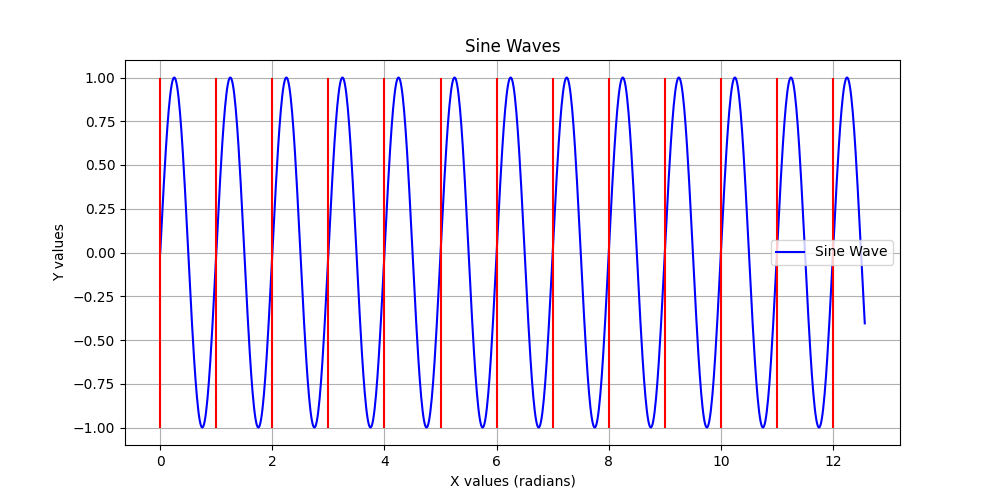
\includegraphics[width=0.9\textwidth,height=0.7\textheight,keepaspectratio]{Figs/sin_waves_exc_613.png}
\end{center}
\begin{center}
    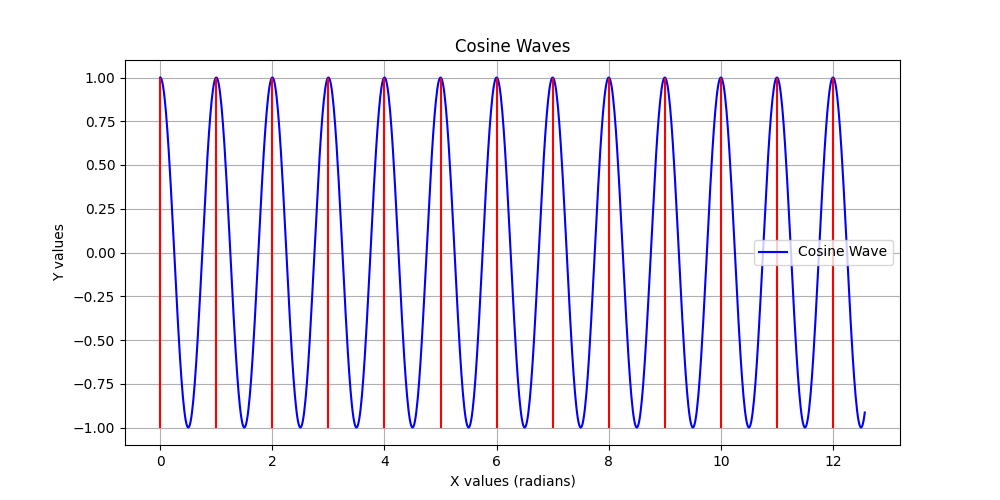
\includegraphics[width=0.9\textwidth,height=0.7\textheight,keepaspectratio]{Figs/cos_waves_exc_613.png}
\end{center}

siden $ k-j  \in \mathbb{Z}$ så vil $ e^{i 2\pi \left( k -j \right) } = 1 $ når $ k \neq j $  og vi får at $ \langle e_k, e_j \rangle_{ L^2 } = 0  $ for $ k\neq j $ og $ \langle e_k, e_j \rangle_{ L^2 } = 1  $ for $ k = j $. dermed er $ \langle e_k, e_j \rangle_{ L^2 } = \delta_{jk}  $ Det integrerte uttrykket $ \frac{ 1 }{ 2\pi } \left[ \frac{ e^{i2\pi \left( k - j \right)  } - 1}{ i \left( k-j \right)  } \right]  $ gjelder bare for når $ k \neq j $. Når $ k=j $, så får vi
\[
    \langle e_k, e_k \rangle_{ L^2 }  = \frac{ 1 }{ 2\pi } \int_{0}^{2\pi} e^{ikt} e^{-ikt}dt = \frac{ 1 }{ 2\pi } \int_{0}^{2\pi} e^0 dt = \frac{ 1 }{ 2\pi } \left[ 2\pi - 0 \right]   = 1
\]
\end{proofbox}   
\end{oppgavebox}


\section*{6.2 Moduloregning og periodiske funksjoner}
\addcontentsline{toc}{section}{6.2 Moduloregning og periodiske funksjoner}

\begin{oppgavebox}{6.2.2}{}
Vis at om f er periodisk med periode am så er også $ f(s + ak) = f(s) \forall k \in \mathbb{Z} $ 

\begin{proofbox}{6.2.2}{}
Her er det nyttig å bruke induksjon
\begin{itemize}
  \item Viser først at for $ P_0 $ er $ f(s + a \cdot 0) = f(s + 0) = f(s) $  
  \item For $ P_1 $ er $ f(s + a \cdot 1) = f(s+a) = f(s) $  er sant av definisjonen til en periodisk funksjon
  \item Anta at $ P_k $  er sann for en $ k \geq 1 $. Hypotesen er at $ f(s + ak) = f(s)  $ for en $ k \in \mathbb{Z} $ 
  \item Vil vise at $ P_{k+1}: f(s + a \left( k+1 \right) ) = f(s) $
  \begin{align*}
    f(s + a \left( k+1 \right)) &= f( \left( s + ak \right) + a) \\
    &=   f \left( s + ak \right) \text{ Dette kommer av definosjonen til en periodisk funksjon } f(s+a) = f(s) \\
    &= f \left( s + ak \right) = f(s) \text{ Her bruker vi hypotesen vår} 
  \end{align*}
  
\end{itemize}
\end{proofbox}
\end{oppgavebox}

\begin{oppgavebox}{6.2.3}{}
La $ k \in \mathbb{Z} $. Vis at funksjonene 
\begin{itemize}
  \item $ f_k(t) := e^{ikt} $
  \item $ g_k(t) := \cos(kt)   $  
  \item $ h_k(t) := \sin(kt)  $ 
\end{itemize}
er $ 2\pi $ periodiske


\begin{proofbox}{6.2.3}{}
\begin{itemize}
  \item Vi begynner med $ f_k(t) = e^{ikt} $. Må vise at 
  \[
      f_k(t+ 2\pi) = f_k(t) \rightarrow e^{ik \left( t + 2\pi \right) } = e^{ikt}
  \]

  \begin{align*}
    e^{ik \left( t + 2\pi \right) } &= e^{ikt} e^{ik2\pi}
  \end{align*}
  \[
      e^{ik2\pi}  = \cos(k2\pi)  + i \sin(k2\pi) 
  \]
  Vi vet at $ \cos(k 2\pi)   $ for en $ k \in \mathbb{Z} $ gir $ \cos(k 2\pi) =1  \forall k \in \mathbb{Z}$ og at $ \sin(2k \pi) = 0 \forall k \in \mathbb{Z}  $. Dermed er
  \[
      e^{ik2\pi} = 1 \forall k \in  \mathbb{Z}
  \]
  Dermed er 
  \begin{align*}
    e^{ik \left( t + 2\pi \right) } &= e^{ikt} e^{ik2\pi}\\
    &= e^{ikt} \cdot 1\\
    &= e^{ikt}
  \end{align*}
  og jeg har vist at $ f_k(t) = e^{ikt} $  er en periodisk funksjon
  \item Vi har nå $ g_k(t) = \cos(kt)   $. Skal så vise at $ \cos(k \left( t+2\pi \right) ) = \cos(kt)     $. 
  \[
      \cos(kt)  = \frac{ e^{ikt} + e^{-ikt}  }{ 2 }
  \]
  Dermed blir 
  \begin{align*}
    \cos(k \left( t + 2\pi \right) )  &= \frac{ e^{ik \left( t + 2\pi \right) } + e^{-ik \left( t + 2 \pi  \right) }   }{ 2 }\\
    &= \frac{ e^{ikt} e^{ik2 \pi } + e^{-ikt} e^{-ik2 \pi }   }{ 2}\\
    &= \frac{ e^{ikt} \cdot 1 + e^{-ikt} \cdot 1 }{ 2 } \\
    &= \frac{ e^{ikt} + e^{-ikt}  }{ 2 } \\
    &= \cos(kt)  
  \end{align*}
  
  \item Og nå tar vi siste $ h_k(t) = \sin(kt)  $. Skal vise at $ \sin(k \left( t + 2 \pi  \right) ) = \sin(kt)   $. Har oppgitt at
  \[
      \sin(kt) = \frac{ e^{ikt} - e^{-ikt}  }{ 2i }
  \]
  
  
  \begin{align*}
    \sin(k \left(  t + 2 \pi  \right) ) &= \frac{ e^{ik \left( t + 2 \pi  \right) - e^{-ik \left( t + 2 \pi  \right) }  }  }{ 2i }\\
    &= \frac{ e^{ikt} e^{ik2 \pi } - e^{-ikt} e^{-ik 2 \pi } }{ 2i}\\
    &= \frac{ e^{ikt} \cdot 1 - e^{-ikt} \cdot 1 }{ 2i }\\
    &= \frac{ e^{ikt} - e^{-ikt}  }{ 2i }\\
    &= \sin(kt) 
  \end{align*}
\end{itemize}
Det er greit å forklare at $ e^{-ikt} = 1  \forall k \in \mathbb{Z}$ fordi du kan bare gå bakover i negativ vinkelretning på enhetssirkelen
\end{proofbox}
\end{oppgavebox}

\begin{oppgavebox}{6.2.10}{}
Finn fourierrekkene til følgende funksjoner
\begin{itemize}
  \item a) $ f: \mathbb{T} \rightarrow \mathbb{R} $ gitt ved $ f(t) = 1 $  
  \item b) $ f: \mathbb{T} \rightarrow \mathbb{R} $ gitt ved $ f(t) = t^2 $ for $ t \in \left[ -\pi, \pi \right)  $   
  \item c) $ f: \mathbb{T} \rightarrow \mathbb{R} $ gitt ved $ f(t) = e^{t}  $ for $ t \in \left[ 0, 2 \pi \right) $ 
\end{itemize}


\begin{proofbox}{6.2.10 a)}{}
Vi finner fourier rekken ved å finne fourier koeffisientene
\[
    \hat{f}_k = \langle f, e_k \rangle_{ L^2 } 
\]
og setter de inn i den generelle formen
\[
    f(t) = \sum_{ k =-n }^{ n } \hat{f}_k e_k
\]
\begin{align*}
  \hat{f}_k &= \frac{ 1 }{ 2 \pi } \int_{0}^{2 \pi 
  } e_0 \overline{e_k} dt \\
  &= \frac{ 1 }{ 2 \pi  }  \int_{0}^{2 \pi } e^{-ikt} dt \\  
  \frac{ 1 }{ 2 \pi  } \int_{0 }^{2 \pi } e^{-ikt} dt &=   \frac{ 1 }{ 2 \pi  } \left[ \frac{ -1 }{ ik } e^{-ikt}  \right]  _0^{2 \pi } \\
  &= \frac{ -1 }{ ik 2 \pi  } \left[ e^{-ik2 \pi } - 1  \right] \\
  &= 0
\end{align*}

Jeg bruker at $ f(t) = e_0 $ fordi det er den nærmeste projeksjonen av f ned på den ortonormale basises $ \left( e_k \right) _{k \in \mathbb{Z}} $. Dette er fordi $ e_0 = e^{ik \cdot 0} = 1 = f(t)  $\\

Så fourierrekken er \[
    f(t) = 1
\]

\end{proofbox}

\begin{proofbox}{6.2.10 b)}{}


Vi bruker det ortonormale basiset $e_k(t) = e^{ikt}$, $k \in \mathbb{Z}$, med indreprodukt:
\[
\langle f, g \rangle = \frac{1}{2\pi} \int_{-\pi}^{\pi} f(t) \overline{g(t)}  dt
\]

Fourier-koeffisientene er gitt ved:
\[
\hat{f}(k) = \langle f, e_k \rangle = \frac{1}{2\pi} \int_{-\pi}^{\pi} t^2 e^{-ikt}  dt
\]

Utregning av koeffisienter

\paragraph{Tilfelle $k = 0$:}
\[
\hat{f}(0) = \frac{1}{2\pi} \int_{-\pi}^{\pi} t^2  dt 
= \frac{1}{2\pi} \left[ \frac{t^3}{3} \right]_{-\pi}^{\pi}
= \frac{1}{2\pi} \cdot \frac{\pi^3 - (-\pi)^3}{3}
= \frac{1}{2\pi} \cdot \frac{2\pi^3}{3}
= \frac{\pi^2}{3}
\]

\paragraph{Tilfelle $k \neq 0$:}
La $I = \int_{-\pi}^{\pi} t^2 e^{-ikt}  dt$. Integrerer ved deler:
\begin{align*}
\text{La: } & u = t^2, \quad dv = e^{-ikt}dt \\
& du = 2tdt, \quad v = \frac{e^{-ikt}}{-ik}
\end{align*}
\begin{align*}
I &= \left[ t^2 \cdot \frac{e^{-ikt}}{-ik} \right]_{-\pi}^{\pi} 
   - \int_{-\pi}^{\pi} \frac{e^{-ikt}}{-ik} \cdot 2t  dt \\
&= \frac{-1}{ik} \left[ t^2 e^{-ikt} \right]_{-\pi}^{\pi} 
   + \frac{2}{ik} \int_{-\pi}^{\pi} t e^{-ikt}  dt
\end{align*}

Grensebidrag:
\[
\left[ t^2 e^{-ikt} \right]_{-\pi}^{\pi} = \pi^2 e^{-ik\pi} - \pi^2 e^{ik\pi} 
= \pi^2(e^{-ik\pi} - e^{ik\pi}) = \pi^2(-2i\sin(k\pi)) = 0
\]
siden $\sin(k\pi) = 0$ for $k \in \mathbb{Z}$.

Dermed:
\[
I = \frac{2}{ik} \int_{-\pi}^{\pi} t e^{-ikt}  dt
\]

Integrerer $\int t e^{-ikt}  dt$ ved deler:
\begin{align*}
\text{La: } & u = t, \quad dv = e^{-ikt}dt \\
& du = dt, \quad v = \frac{e^{-ikt}}{-ik}
\end{align*}
\begin{align*}
\int_{-\pi}^{\pi} t e^{-ikt}  dt &= \left[ t \cdot \frac{e^{-ikt}}{-ik} \right]_{-\pi}^{\pi} 
- \int_{-\pi}^{\pi} \frac{e^{-ikt}}{-ik}  dt \\
&= \frac{-1}{ik} \left[ t e^{-ikt} \right]_{-\pi}^{\pi} 
+ \frac{1}{ik} \int_{-\pi}^{\pi} e^{-ikt}  dt
\end{align*}

Grensebidrag:
\[
\left[ t e^{-ikt} \right]_{-\pi}^{\pi} = \pi e^{-ik\pi} - (-\pi)e^{ik\pi} 
= \pi(e^{-ik\pi} + e^{ik\pi}) = 2\pi\cos(k\pi)
\]

Integralet:
\[
\int_{-\pi}^{\pi} e^{-ikt}  dt = \left[ \frac{e^{-ikt}}{-ik} \right]_{-\pi}^{\pi} 
= \frac{e^{-ik\pi} - e^{ik\pi}}{-ik} = \frac{-2i\sin(k\pi)}{-ik} = 0
\]

Dermed:
\[
\int_{-\pi}^{\pi} t e^{-ikt}  dt = \frac{-1}{ik} \cdot 2\pi\cos(k\pi) = \frac{-2\pi\cos(k\pi)}{ik}
\]

Setter inn i $I$:
\[
I = \frac{2}{ik} \cdot \frac{-2\pi\cos(k\pi)}{ik} 
= \frac{-4\pi\cos(k\pi)}{i^2 k^2} 
= \frac{-4\pi\cos(k\pi)}{-k^2} 
= \frac{4\pi\cos(k\pi)}{k^2}
\]

Fourier-koeffisient for $k \neq 0$:
\[
\hat{f}(k) = \frac{1}{2\pi} \cdot I = \frac{1}{2\pi} \cdot \frac{4\pi\cos(k\pi)}{k^2} 
= \frac{2\cos(k\pi)}{k^2}
\]

Resultatet blir så

Fourier-koeffisienter:
\[
\hat{f}(k) = 
\begin{cases}
\dfrac{\pi^2}{3}, & k = 0 \\[1em]
\dfrac{2\cos(k\pi)}{k^2}, & k \neq 0
\end{cases}
\]

Fourier-rekke (kompleks form):
\[
t^2 \sim \sum_{k=-\infty}^{\infty} \hat{f}(k)e^{ikt} 
= \frac{\pi^2}{3} + \sum_{\substack{k=-\infty \\ k \neq 0}}^{\infty} \frac{2\cos(k\pi)}{k^2} e^{ikt}
\]
\end{proofbox}

\begin{proofbox}{6.2.10 c)}{}


Fourier-rekke for $f(t) = e^t$ på $[-\pi,\pi)$

Vi bruker det ortonormale basiset $e_k(t) = e^{ikt}$, $k \in \mathbb{Z}$, med indreprodukt:
\[
\langle f, g \rangle = \frac{1}{2\pi} \int_{-\pi}^{\pi} f(t) \overline{g(t)}  dt
\]

Fourier-koeffisientene er gitt ved:
\[
\hat{f}(k) = \langle f, e_k \rangle = \frac{1}{2\pi} \int_{-\pi}^{\pi} e^{t} e^{-ikt}  dt
= \frac{1}{2\pi} \int_{-\pi}^{\pi} e^{(1 - ik)t}  dt
\]

Utregning av koeffisienter

La $\alpha = 1 - ik$. Da har vi:
\[
\hat{f}(k) = \frac{1}{2\pi} \int_{-\pi}^{\pi} e^{\alpha t}  dt
\]

Regner ut integralet:
\[
\int_{-\pi}^{\pi} e^{\alpha t}  dt = \left[ \frac{e^{\alpha t}}{\alpha} \right]_{-\pi}^{\pi}
= \frac{e^{\alpha \pi} - e^{-\alpha \pi}}{\alpha}
\]

Dermed:
\[
\hat{f}(k) = \frac{1}{2\pi} \cdot \frac{e^{\alpha \pi} - e^{-\alpha \pi}}{\alpha}
= \frac{e^{\alpha \pi} - e^{-\alpha \pi}}{2\pi \alpha}
\]

Setter inn $\alpha = 1 - ik$:
\[
\hat{f}(k) = \frac{e^{(1 - ik)\pi} - e^{-(1 - ik)\pi}}{2\pi (1 - ik)}
\]

Forenkler telleren:
\[
e^{(1 - ik)\pi} = e^{\pi} e^{-ik\pi} = e^{\pi} [\cos(k\pi) - i\sin(k\pi)] = e^{\pi} \cos(k\pi)
\]
\[
e^{-(1 - ik)\pi} = e^{-\pi} e^{ik\pi} = e^{-\pi} [\cos(k\pi) + i\sin(k\pi)] = e^{-\pi} \cos(k\pi)
\]

Dermed:
\[
e^{(1 - ik)\pi} - e^{-(1 - ik)\pi} = (e^{\pi} - e^{-\pi}) \cos(k\pi) = 2\sinh(\pi) \cos(k\pi)
\]

Resultatet blir så

Fourier-koeffisienter:
\[
\hat{f}(k) = \frac{2\sinh(\pi) \cos(k\pi)}{2\pi (1 - ik)}
= \frac{\sinh(\pi) \cos(k\pi)}{\pi (1 - ik)}
\quad \text{for alle } k \in \mathbb{Z}
\]

Fourier-rekke (kompleks form):
\[
e^t \sim \sum_{k=-\infty}^{\infty} \hat{f}(k)e^{ikt} 
= \sum_{k=-\infty}^{\infty} \frac{\sinh(\pi) \cos(k\pi)}{\pi (1 - ik)} e^{ikt}
\]

Alternativt kan vi skrive dette som:
\[
e^t \sim \frac{\sinh(\pi)}{\pi} \sum_{k=-\infty}^{\infty} \frac{\cos(k\pi)}{1 - ik} e^{ikt}
\]


\end{proofbox}
\end{oppgavebox}



\end{document}